\documentclass[preprint]{elsarticle}
\usepackage{hyperref}
\usepackage{amsmath}
\usepackage{url}
\usepackage[spanish]{babel}
\usepackage[utf8]{inputenc}
\usepackage{graphicx}
\usepackage{float}


\bibliographystyle{model2-names}


\begin{document}

\begin{frontmatter}

\title{Algunas gráficas para mapas logísticos}


\author[md]{Marcos Daniel Calderón-Calderón}



\address[md]{Center for Research in Mathematics (CIMAT), Guanajuato, México.}


\begin{abstract}
Se muestran algunas gráficas para el mapa logístico.
\end{abstract}



\end{frontmatter}



 
   
 
 






\section{Graficas de ocho mapas acoplados}
\label{ac}

En este esquema cambia más la manera en cómo se aplica la operación XOR: el contador aumenta en uno; además, se aplica la operación XOR dos veces: la primera vez es un recorrido de izquierda a derecha, la segunda vez es un recorrido de derecha a izquierda. La distribucion de los valores obtenidos se muestran en la figura~\ref{fbl} y en la figura~\ref{fbd}.


\begin{figure}[H]  
\centering
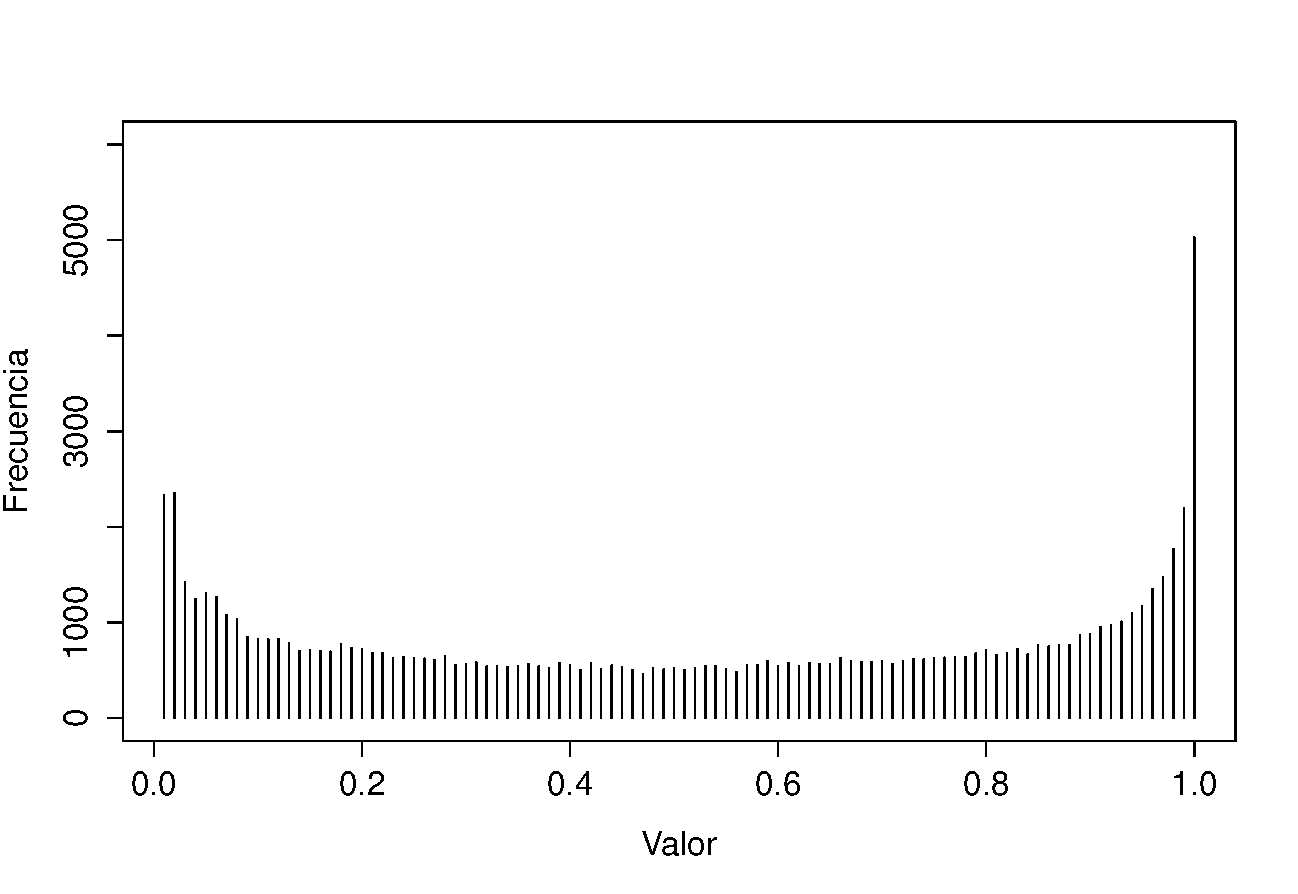
\includegraphics[width=8cm]{fbl2.pdf}
\caption{Histograma de los valores generados en el esquema 5B.}
\label{fbl}
\end{figure}


\begin{figure}[H]
\centering
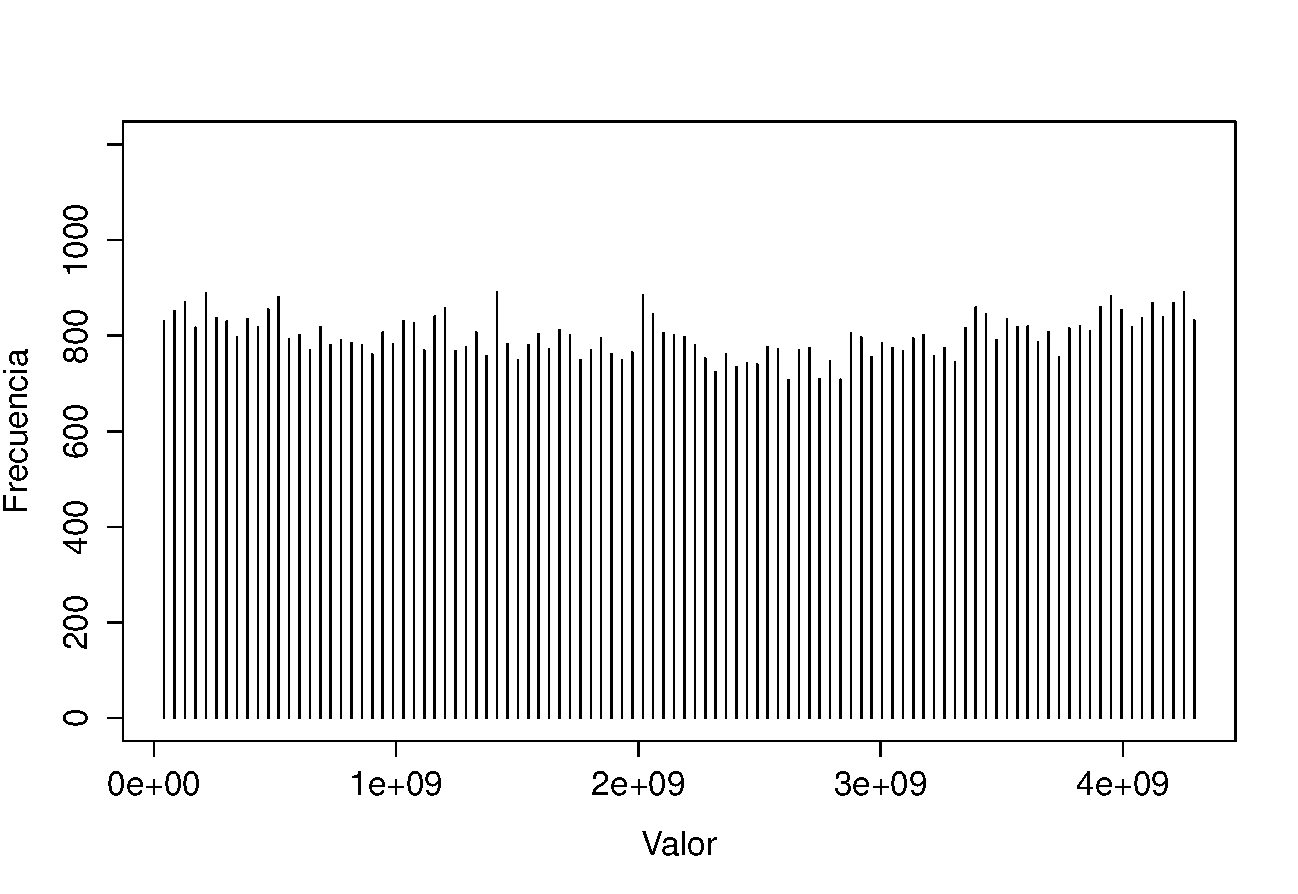
\includegraphics[width=8cm]{fbd2.pdf}
\caption{Histograma de valores caóticos discretizados para el esquema 5B.}
\label{fbd}
\end{figure}







\end{document}